%!TEX root = ../Hardtung_BA_SoSe20.tex

\section{Problems \& other Findings}
\label{sec:problems}

This section discusses decisions and problems during the development process.


\subsection{Virtual Folding}

Simulating the folding of paper for origami models by the Origrammer has introduced a multitude of edgecases and constraints that have to be kept track of, in order to present a correct and predictable result.

\subsubsection{Folding over and over}

Making simple valley or mountain folds where only one layer of the paper is being folded (e.g. folding the corner of the paper), does not introduce many constraints. Internally, the Origrammer just has to split the existing polygon on the folding line and then update the position (fold) of one of these split up polygons with the folding line as the base.

Though as soon as there are multiple polygons connected to the newly made crease line, more calculations will have to be carried out. Especially, once the user wants to fold over and over to create multiple layers of paper (as seen in Figure \ref{fig:foldingMultipleLinkedPolygons}), all the affected polygons are influencing the resulting layer height of each other.
\begin{figure}[htbp]
	\centering
	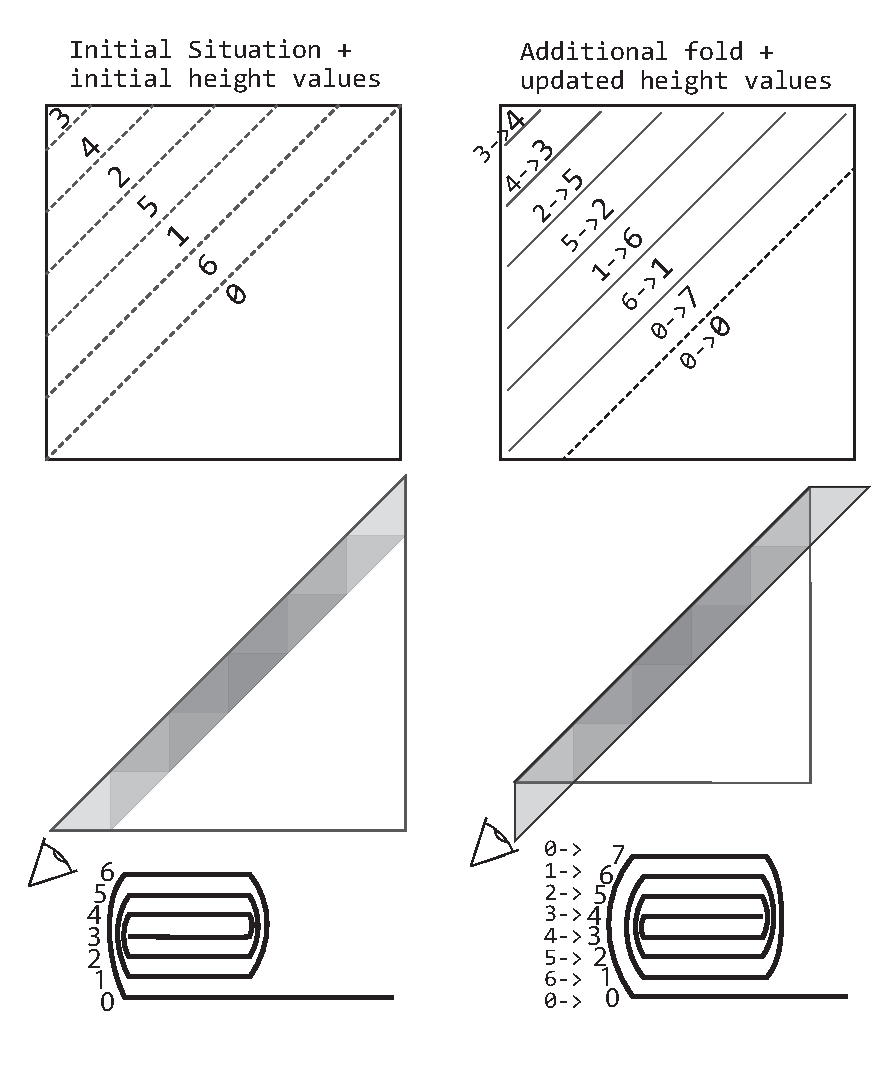
\includegraphics[width=0.8\textwidth]{foldingMultipleLinkedPolygons}
	\caption{Folding the paper over and over - Folding Polygons that don't share a line with the folding line}
	\label{fig:foldingMultipleLinkedPolygons}
\end{figure}

% p0-p7   --> 
% p0+1   p1-1
% p2+3   p2-3
% p4+5   p5-5
% p6-7    p7-7

\begin{lstlisting}[label=oriPolygon,caption=OriPolygon]
ArrayList<OriPolygon> sortedPolygons;
int curLowHeight = hmin; //1
int curUpHeight = hmax; //7
boolean justDidUpper = false;

for (OriPolygon curP : sortedPolygons) {
    if (!justDidUpper) {
        curP.setHeight(curUpHeight);
        curUpHeight -= 1; //goes lower for every 2nd folded polygon
        justDidUpper = true;
    } else {
        curP.setHeight(curLowHeight);
        curLowHeight += 1; //goes higher for every 2nd folded polygon
        justDidUpper = false;
    }
}
\end{lstlisting}




\subsection{Folding multiple layers}

Another problematic scenario arises once the user wants to fold through multiple independent layers. Independ from each other means in this case, that the polygons that represent these layers can be folded independently from each other. This situation can be seen in Figure \ref{fig:foldingMultipleLayersAtSameTime} where the two corners facing the top right are to be folded downwards. 

\begin{figure}[htbp]
	\centering
	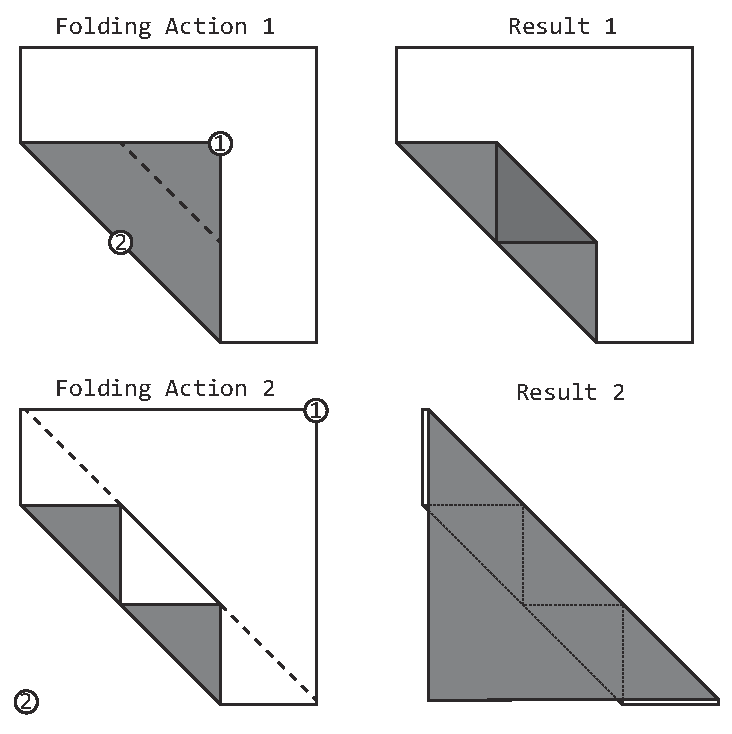
\includegraphics[width=0.7\textwidth]{foldingMultipleLayersAtSameTime}
	\caption{Folding through multiple independend layers at the same time}
	\label{fig:foldingMultipleLayersAtSameTime}
\end{figure}

\noindent Currently, the user would have to carry out these folding actions one by one and the Origrammer would create 2 seperate folding steps. This situation arises because the Origrammer only folds all connected layers looking from the top layer. But as the inputted folding line crosses edge lines on both sides of this top polygon, it is the only layer being folded.\\
Additionally in this specific example, there is no clear reference point where the second folding action should end (point 2 at Folding Action 2). This is compared to the first folding action, where the corner simply gets folded towards an outer edge line.


\noindent In order to increase efficiency and to remove this edgecase of missing reference points, a feature should be implemented, where the user can specify through how many layers the folding step should fold through.%Only for efficiency's sake and not to an error in the virtual folding
